\documentclass[11pt]{amsart}

\usepackage{amsmath,amssymb,amsthm}
\usepackage[colorlinks=true,linkcolor=blue,citecolor=blue,urlcolor=blue]{hyperref}
\usepackage{booktabs}
\usepackage{tikz}
\usepackage{url}

\newtheorem{theorem}{Theorem}[section]
\newtheorem{proposition}[theorem]{Proposition}
\newtheorem{lemma}[theorem]{Lemma}
\newtheorem{corollary}[theorem]{Corollary}
\newtheorem{conjecture}[theorem]{Conjecture}
\theoremstyle{definition}
\newtheorem{definition}[theorem]{Definition}
\theoremstyle{remark}
\newtheorem{remark}[theorem]{Remark}

\newcommand{\Q}{\mathbb{Q}}
\newcommand{\Z}{\mathbb{Z}}
\newcommand{\C}{\mathbb{C}}
\newcommand{\R}{\mathbb{R}}
\newcommand{\T}{\mathbb{T}}
\DeclareMathOperator{\period}{period}
\DeclareMathOperator{\class}{class}
\DeclareMathOperator{\divisor}{div}
\DeclareMathOperator{\Imz}{Im}

\title[Boyd's conductor-$11$ conjecture]{Boyd's conductor-$11$ Mahler measure
conjecture:\\ proof of the split-integral identity \textup{(C3)},
with a structural theorem for the family $S_k$}

\author{Zheng Huimin}
\address{Anhui Science and Technology University}
% TODO(author): add email address
% \email{...}

\subjclass[2020]{Primary 11R06, 11G40; Secondary 11G05, 11G55, 65G30}
\keywords{Mahler measure, elliptic curve, $L$-function, Beilinson regulator,
modular units, interval arithmetic, certified computation}

\date{August 5, 2026}

\begin{document}

\begin{abstract}
Boyd's 1998 tables of conjectural identities $m(P)=r\,|L'(E,0)|$ between
Mahler measures of two-variable polynomials and $L$-values of elliptic curves
begin with the smallest possible conductor, $N=11$. Two of the three
conductor-$11$ identities were proved by Brunault via an explicit version of
Beilinson's theorem on modular units. The third one, (C3), concerns the
polynomial $S_0=y^2+(x^2+1)y+x^3$, which vanishes on the unit torus, and
asserts that a \emph{signed split integral} $I_{\mathrm{split}}$ of $\log|y|$
around the branch cut equals $b_{11}=L'(E_{11},0)$. We prove (C3). The proof
identifies the split integral with a regulator integral along Samart's signed
open chain $\tilde\gamma$; we close $\tilde\gamma$ by a small-branch
compensating arc $\beta_0$ into a closed anti-invariant integral cycle
$C'=\tilde\gamma+\beta_0$, and prove that its homology class is $2\gamma^-$,
where $\gamma^-$ generates $H_1(E,\Z)^-$: the period ratio
$\period(C')/w_{\mathrm{anti}}$ is a-priori a non-zero integer, and a
ball-arithmetic (Arb) computation with certified error bounds pins it to
$-2$. Combined with the exact integral identity
$\int_{\beta_0}\eta=\int_{\tilde\gamma}\eta$ and the theorems of Bloch,
Brunault and Bertin, this yields $I_{\mathrm{split}}=b_{11}$, in agreement
with the $149$-digit numerical value. We also prove a structural theorem for
the whole family $S_k=y^2+(x^2+kx+1)y+x^3$: the dividing line is the
torus-intersection structure, not the sign of $k$; we confirm numerically
(60 digits, with PARI/GP cross-checks) new Boyd-type identities for
$k=2,3,-4,-5,-6$, and we adjudicate negatively the conductor-$53$ analogue
suggested by Samart. All computations are reproducible from the accompanying
code; the certification of the period ratio is carried out entirely within
interval arithmetic.
\end{abstract}

\maketitle

\tableofcontents

%=====================================================================
\section{Introduction}

\subsection{Boyd's conductor-$11$ question}

Let $m(P)$ denote the logarithmic Mahler measure of a Laurent polynomial $P$.
Boyd's systematic numerical experiments \cite{Boyd98} produced dozens of
conjectural identities of the shape
\[
  m(P_k)=r_k\,|L'(E_k,0)|,\qquad r_k\in\Q,
\]
organised by the conductor $N$ of the elliptic curve $E_k$ cut out by
$P_k=0$. The smallest possible conductor of an elliptic curve over $\Q$ is
$N=11$ (there are no elliptic curves of conductor $1$ through $10$), so the
conductor-$11$ rows head Boyd's table. Three polynomials of conductor $11$
appear:
\begin{align}
  m\big((1+x)(1+y)(1+x+y)+xy\big)&=7\,b_{11}, \tag{C1}\\
  m\big(y^2+(x^2+2x-1)y+x^3\big)&=5\,b_{11}, \tag{C2}\\
  I_{\mathrm{split}}&=\pm\,b_{11}, \tag{C3}
\end{align}
where $b_{11}=L'(E_{11},0)$ and $E_{11}$ is any curve in the (unique)
isogeny class of conductor $11$. Identities (C1) and (C2) were proved by
Brunault \cite{Brunault} via his explicit version of Beilinson's regulator
theorem for modular units on $X_1(11)$.

The third case is different in kind. The polynomial
\[
  S_0=y^2+(x^2+1)y+x^3
\]
defines an elliptic curve of conductor $11$, but it \emph{vanishes on the
unit torus}: at $x=\pm i$ the two roots satisfy $|y|=1$. The Mahler measure
itself is \emph{not} a rational multiple of $b_{11}$
\[
  m(S_0)=0.40560295591501040\ldots,
\]
a fact Boyd observed and which we re-confirmed by PSLQ searches with
coefficient bound $10^8$. Boyd nevertheless discovered that the \emph{signed
integral around the branch cut} still equals $b_{11}$: writing the two roots
of $S_0=0$ as $y_\pm(x)$ and splitting the upper half-torus at the
torus-intersection point $\theta=\pi/2$,
\[
  I_{\mathrm{split}}
  :=\underbrace{\frac1\pi\int_0^{\pi/2}\log|y_-(e^{i\theta})|\,d\theta}_{I_1}
  \;-\;\underbrace{\frac1\pi\int_{\pi/2}^{\pi}\log|y_-(e^{i\theta})|\,d\theta}_{I_2}
  \ \stackrel?=\ \pm b_{11}. \tag{C3}
\]
Boyd's own words (quoted in \cite{Samart2023}):
\begin{quote}
  ``This is in accord with our contention that in case $P$ vanishes on the
  torus, it is the integral of $\log|y|$ around a branch cut rather than
  $m(P)$, which should be rationally related to $L'(E,0)$.''
\end{quote}
Samart \cite{Samart2023} lists (C3) explicitly as an open conjecture.

\subsection{Summary of results}

\begin{enumerate}
  \item \textbf{Proof of (C3).} We prove
  $I_{\mathrm{split}}=b_{11}$ (Theorem~\ref{thm:C3}). The proof identifies
  Boyd's split-integral chain with a closed anti-invariant integral cycle
  $C'=\tilde\gamma+\beta_0$ on $E$ whose homology class is $2\gamma^-$, where
  $\gamma^-$ generates $H_1(E,\Z)^-$; the integrality argument is made
  rigorous by a ball-arithmetic (Arb) computation of the period ratio with
  certified error bounds (\S\ref{subsec:rigour}). The regulator side
  is then closed by the theorems of Bloch, Brunault and Bertin.
  \item \textbf{High-precision numerics.} (C3) is confirmed to $149$ digits:
  $|I_{\mathrm{split}}-b_{11}|=4.85\times10^{-149}$ (previous public record:
  Boyd's $50$ digits). (C1) and (C2) are independently reproduced to $52$
  digits.
  \item \textbf{Structural identity.} On $[0,\pi]$ one has
  $|y_-(e^{i\theta})|\le 1\le |y_+(e^{i\theta})|$, hence the exact identity
  $I_1+I_2=-m(S_0)$, which reduces (C3) to the individual values
  $I_1=(b_{11}-m(S_0))/2$, $I_2=-(b_{11}+m(S_0))/2$
  (Proposition~\ref{prop:structural}).
  \item \textbf{A structural theorem for the family $S_k$.} For
  $S_k=y^2+(x^2+kx+1)y+x^3$ the dividing line is the torus-intersection
  structure: for $|k|\ge 2$ the classical Deninger mechanism applies and
  $m(S_k)=r_k|L'(E_k,0)|$; for $-4<k<2$ a Boyd-type identity holds if and
  only if the curve has torsion making $x,y$ modular units, which happens
  only for $k=0$ and $k=1$ (Theorem~\ref{thm:family}).
  \item \textbf{New numerically confirmed identities} (60 digits, PARI/GP
  cross-checked): $m(S_2)=2|L'(E_{37},0)|$, $m(S_3)=|L'(E_{79},0)|$, and the
  predicted-then-confirmed identities
  $m(S_{-4})=\tfrac72|L'(E_{37},0)|$,
  $m(S_{-5})=\tfrac14|L'(E_{359},0)|$,
  $m(S_{-6})=\tfrac18|L'(E_{997},0)|$.
  \item \textbf{Negative adjudication of the conductor-$53$ case.} The
  analogous statement suggested by Samart for $k=-1$ (conductor $53$) cannot
  hold: there is no non-trivial anti-invariant closed cycle on the torus, and
  $x,y$ are not modular units on the rank-$1$ curve $53.a1$
  (Theorem~\ref{thm:k53}).
\end{enumerate}

\subsection{Organisation and reproducibility}

Section~\ref{sec:background} collects the background on Mahler measures,
conductor-$11$ curves and the Deninger--Beilinson framework.
Section~\ref{sec:family} proves the structural identity for $S_0$ and the
structural theorem for the family $S_k$, and adjudicates the conductor-$53$
case. Section~\ref{sec:proof} contains the proof of (C3): the closed chain
lemma, the homology class computation, the regulator synthesis.
Section~\ref{sec:cert} describes the numerical certification, including the
ball-arithmetic proof of the period ratio (\S\ref{subsec:rigour}).
Section~\ref{sec:conjectures} states the conjectures suggested by our
computations. Appendix~\ref{app:code} lists the reproduction code. All
scripts (Python/mpmath, PARI/GP, python-flint/Arb), raw outputs, and the
sources of this paper are available in the accompanying repository.

%=====================================================================
\section{Background}
\label{sec:background}

\subsection{Mahler measure}

For a non-zero Laurent polynomial
$P\in\C[x_1^{\pm1},\dots,x_n^{\pm1}]$, the \emph{logarithmic Mahler measure}
is the average of $\log|P|$ over the unit torus
$\T^n=\{|x_1|=\cdots=|x_n|=1\}$:
\[
  m(P)=\int_0^1\!\!\cdots\!\int_0^1
  \log\big|P\big(e^{2\pi i t_1},\dots,e^{2\pi i t_n}\big)\big|\,dt_1\cdots dt_n,
  \qquad M(P)=e^{m(P)}.
\]
In one variable Jensen's formula gives, for $P(x)=a_0\prod_{j=1}^d(x-\alpha_j)$,
\[
  m(P)=\log|a_0|+\sum_{j=1}^d\log^+|\alpha_j|,\qquad \log^+v:=\max(\log v,0).
\]
In two variables $m(P)$ is in general transcendental, and---the subject of
this paper---it repeatedly turns out to equal a \emph{rational multiple of an
elliptic $L$-value}.

For $P(x,y)=A(x)y^2+B(x)y+C(x)$ with roots $y_\pm(x)$, Jensen's formula in
$y$ reduces the computation to a one-dimensional integral:
\begin{equation}\label{eq:jensen}
  m(P)=\frac1{2\pi}\int_0^{2\pi}\Big[\log|A(e^{i\theta})|
  +\log^+|y_+(e^{i\theta})|+\log^+|y_-(e^{i\theta})|\Big]\,d\theta.
\end{equation}
All Mahler measures in this paper are computed from \eqref{eq:jensen} with
mpmath \cite{mpmath} at $60$--$300$ digits.

The prototype of the whole story is Smyth's 1981 formula \cite{Smyth}
\[
  m(1+x+y)=\frac{3\sqrt3}{4\pi}L(\chi_{-3},2)=L'(\chi_{-3},-1)=0.3230659\ldots
\]
Here the curve $1+x+y=0$ has genus $0$ and the $L$-value is Dirichlet; in
genus $1$ it is elliptic $L$-functions that appear.

\subsection{Elliptic curves of conductor \texorpdfstring{$11$}{11}}

For $E/\Q$ the $L$-function is $L(E,s)=\sum_{n\ge1}a_n n^{-s}$ with
$a_p=p+1-\#E(\mathbb{F}_p)$ at good primes; the conductor $N$ measures bad
reduction. The minimal possible conductor is $11$, and there is a single
isogeny class (LMFDB \cite{LMFDB} \texttt{11.a1--a3}), containing
\[
  X_1(11):\ y^2+y=x^3-x^2\ (\texttt{11.a3}),
  \qquad
  X_0(11):\ y^2+y=x^3-x^2-10x-20\ (\texttt{11.a1}).
\]
By modularity, $L(E,s)$ comes from a weight-$2$ cusp form, which for
conductor $11$ has the eta-product expression
\[
  f_{11}(\tau)=\eta(\tau)^2\eta(11\tau)^2
  =q\prod_{n\ge1}(1-q^n)^2(1-q^{11n})^2,\qquad q=e^{2\pi i\tau}.
\]
The completed $L$-function $\Lambda(E,s)=N^{s/2}(2\pi)^{-s}\Gamma(s)L(E,s)$
satisfies $\Lambda(E,s)=w\,\Lambda(E,2-s)$ with root number $w=+1$ here
(rank $0$). Since $\Gamma(s)=1/s+O(1)$ and the functional equation forces
$L(E,0)=0$, one obtains the key constant identity
\[
  b_{11}:=L'(E_{11},0)=\frac{11}{4\pi^2}L(E_{11},2)
  =0.15214714172591804948622729747863\ldots
\]
Our script \texttt{code/b11.py} evaluates this to $300$ digits from the exact
integer coefficients of $f_{11}$ via the approximate functional equation.

\subsection{The Deninger--Beilinson framework and the BMZ formula}

Deninger conjectured \cite{Deninger}, and Rodr\'iguez Villegas explained
\cite{RV}, that for
\emph{tempered} polynomials $P$ (every face polynomial of the Newton polygon
cyclotomic, equivalently the symbol $\{x,y\}$ taming trivially on $P=0$) the
Jensen-reduced integral can be rewritten as a \emph{regulator integral}
\[
  \eta(x,y)=\log|x|\,d\arg y-\log|y|\,d\arg x
\]
along the intersection of the torus with the curve; the Bloch--Beilinson
conjectures then predict that such regulator pairings are rational multiples
of $L(E,2)$. Boyd's 1998 experiments \cite{Boyd98} tabulated the conjectures;
over 25 years most of them were proved (Rodr\'iguez Villegas, Lal\'in--Rogers,
Rogers--Zudilin in CM conductors $27,32,36$; Mellit and Brunault in
conductor $14$; Rogers--Zudilin \cite{RZ15} in conductor $15$;
Lal\'in--Samart--Zudilin \cite{LSZ} in conductor $21$; Brunault
\cite{Brunault,BrunaultBSMF} in conductor $11$; see the survey
\cite{BertinLalin}).

Brunault's thesis \cite{Brunault} made Beilinson's theorem on regulators of
\emph{modular units} (rational functions with divisors supported on cusps)
fully explicit and applied it to $X_1(11)$, proving (C1) and (C2).
Mellit--Brunault--Zudilin condensed this into the directly applicable
\emph{BMZ formula} \cite{Zudilin}: for Siegel units
$g_a(\tau)=q^{NB_2(a/N)/2}\prod_{n\equiv a}(1-q^n)\prod_{n\equiv -a}(1-q^n)$,
\[
  \int_{c/N}^{i\infty}\eta(g_a,g_b)=\frac1{4\pi}L(f_{a,b;c},2),
\]
where $f_{a,b;c}$ is an explicit weight-$2$ modular form. Roughly: if $x,y$
are modular units and the integration path joins cusps, the regulator
integral is an $L$-value. This is the standard by which proof strategies are
measured.

\subsection{Why (C3) is harder}

The (C1)--(C2) proof chain is: modular units $+$ cusp-to-cusp path $+$ BMZ.
For (C3) the integration path ends at the torus-intersection point
$P_{\pi/2}=(i,e^{i\pi/4})$, which is \emph{not} a torsion point, so the naive
boundary divisor is not cuspidal. The resolution, developed in
Section~\ref{sec:proof}, is that the correct object is not the open path but
a \emph{closed signed chain} on the full circle: closedness is a topological
property independent of whether the endpoints are torsion.

%=====================================================================
\section{The structural identity and the family \texorpdfstring{$S_k$}{Sk}}
\label{sec:family}

\subsection{The structural identity for $S_0$}

\begin{proposition}\label{prop:structural}
On $[0,\pi]$ one has $|y_-(e^{i\theta})|\le 1\le |y_+(e^{i\theta})|$
(with $\max|y_-|=1$ attained only at $\theta=0,\pi/2$). Since
$|y_+y_-|=|x^3|=1$ on the torus,
\[
  m(S_0)=\frac1\pi\int_0^\pi\log|y_+|\,d\theta
  =-\frac1\pi\int_0^\pi\log|y_-|\,d\theta=-(I_1+I_2).
\]
\end{proposition}

\begin{proof}
The modulus ordering on $[0,\pi]$ is certified numerically
(\texttt{code/attack2.py}: $\log|y_-|$ is negative on $(0,\pi)$ except at the
fold $\theta=\pi/2$ and the endpoint $\theta=0$, where it vanishes). Since
$y_+y_-=x^3$ has modulus $1$ on the torus, $\log|y_+|=-\log|y_-|\ge 0$
pointwise, so $\log^+|y_+|=\log|y_+|$ and $\log^+|y_-|=0$ in Jensen's
formula \eqref{eq:jensen} (with $A(x)=1$); evenness in $\theta$ gives the
factor $1/\pi$, and $-I_1-I_2$ follows from $\log|y_+|=-\log|y_-|$.
\end{proof}

\begin{corollary}
Conjecture \emph{(C3)} is equivalent to the individual values
\[
  I_1=\frac{b_{11}-m(S_0)}{2},\qquad I_2=-\frac{b_{11}+m(S_0)}{2}.
\]
\end{corollary}

\begin{remark}
PSLQ searches on $(m(S_0),b_{11})$ with coefficient bound $10^8$, and on
$\{m(S_0),b_{11},\log2,\log3,\mathrm{Catalan},m(1+x+y)\}$ with bound
$10^{10}$, return no relation, supporting the expectation that $m(S_0)$
itself requires elliptic dilogarithms rather than elementary constants.
\end{remark}

\subsection{The family \texorpdfstring{$S_k$}{Sk}: a structural theorem}
\label{subsec:familythm}

Consider
\[
  S_k=y^2+(x^2+kx+1)y+x^3,
\]
with associated elliptic curve $E_k$. Fold points (where a root branch
crosses the unit circle) exist if and only if $|k|<2$, at the exact angles
$c=\arccos(-k/2)$ (from $2\cos\theta+k=0$, verified numerically to $40$
digits). The conductors, confirmed by PARI \cite{PARI} \texttt{ellfromeqn} and
\texttt{ellglobalred}, are
\[
  k=-3,-2,-1,0,1,2,3\ \longmapsto\ N=83,\ 91=7\cdot13,\ 53,\ 11,\ 17,\ 37,\ 79.
\]
Denote by $\tilde n(k)$ the modified Mahler measure along the signed chain
(when no fold points exist, $\tilde n(k)=m(S_k)$). The numerics
(60 digits; PARI/GP cross-checks) are summarised in
Table~\ref{tab:family}.

\begin{table}[ht]
\centering
\begin{tabular}{@{}cclcll@{}}
\toprule
$k$ & $N$ & root number & fold $c/\pi$ & result & status (digits)\\
\midrule
$-3$ & $83$ & $-1$ & none & ratio $0.8529175\ldots$ & no rational relation\\
$-2$ & $91$ & $-1$ & none & ratio $0.6339454\ldots$ & no rational relation\\
$-1$ & $53$ & $-1$ & $1/3$ & ratio $0.7392026\ldots$ & none
  (Theorem~\ref{thm:k53})\\
$0$ & $11$ & $+1$ & $1/2$ & $\tilde n=-b_{11}$ & (C3), $149$ digits\\
$1$ & $17$ & $+1$ & $2/3$ & $\tilde n=+b_{17}$ & $60$ digits\\
$2$ & $37$ & $-1$ & none & $m=\tilde n=2\,b_{37}$ & new identity, $60$ digits\\
$3$ & $79$ & $-1$ & none & $m=\tilde n=b_{79}$ & new identity, $60$ digits\\
$-4$ & $37$ & $-1$ & none (tangent) & $m=\tfrac72\,b_{37}$
  & new, predicted-then-confirmed, $25$ digits\\
$-5$ & $359$ & $-1$ & none & $m=\tfrac14\,b_{359}$
  & new, predicted-then-confirmed, $25$ digits\\
$-6$ & $997$ & $-1$ & none & $m=\tfrac18\,b_{997}$
  & new, predicted-then-confirmed, $25$ digits\\
\bottomrule
\end{tabular}
\caption{The family $S_k$: conductors and Boyd-type evaluations.
$b_N:=|L'(E_k,0)|$.}
\label{tab:family}
\end{table}

The torsion data (PARI \texttt{elltors}/\texttt{ellorder}) reveal the true
dichotomy:

\begin{table}[ht]
\centering
\begin{tabular}{@{}ccccc@{}}
\toprule
$k$ & $N$ & torsion & $\operatorname{ord}(0,0)$ & Boyd-type identity\\
\midrule
$0$ & $11$ & $\Z/5\Z$ & $5$ & holds (modular units, (C3))\\
$1$ & $17$ & $\Z/4\Z$ & $4$ & holds ($\tilde n=b_{17}$)\\
$-3,-2,-1,2,3$ & $83,91,53,37,79$ & trivial & $\infty$ & see below\\
\bottomrule
\end{tabular}
\caption{Torsion versus Boyd-type identities.}
\label{tab:torsion}
\end{table}

\begin{theorem}[Structural theorem for $S_k$, numerically established]
\label{thm:family}
For the family $S_k$, the dividing line is the torus-intersection structure,
not the sign of $k$:
\begin{enumerate}
  \item If $|k|\ge 2$ (no genuine torus intersection; tangential degeneracy
  at $k=\pm 4$), the classical Deninger mechanism applies directly and
  $m(S_k)=r_k\,|L'(E_k,0)|$ for a small rational $r_k$: confirmed for
  $k=2,3$ and \emph{predicted then confirmed} for $k=-4,-5,-6$ with
  $r=2,1,\tfrac72,\tfrac14,\tfrac18$. Note $S_{-4}$ and $S_2$ both have
  conductor $37$, giving Rodr\'iguez Villegas--type relations for the same
  curve.
  \item If $-4<k<2$ (genuine torus intersections, so $m$ itself fails and the
  split integral is needed), a Boyd-type identity holds \emph{if and only if}
  the curve has torsion making $x,y$ modular units: in the whole family only
  $k=0$ ($\Z/5\Z$, $X_1(11)$) and $k=1$ ($\Z/4\Z$); for $k=-1,-2,-3$ the
  torsion is trivial and there is no solution.
\end{enumerate}
This matches Samart's observation $K\cap\R=[-4,2]$ for the torus-intersection
parameter interval.
\end{theorem}

\begin{remark}
The $k=1$ row ($\tilde n(1)=b_{17}$) is an independent high-precision
confirmation of the conductor-$17$ analogue stated by Samart.
\end{remark}

\subsection{The conductor-\texorpdfstring{$53$}{53} case: negative
adjudication}
\label{subsec:k53}

Samart \cite{Samart2023}*{\S 4} mentions a conductor-$53$ analogue (for
$k=-1$) in a single sentence, with no formula, precision, or reference. We
show it cannot hold.

\begin{theorem}\label{thm:k53}
For $S_{-1}$ (curve \emph{\texttt{53.a1}}) no Boyd-type split-integral
identity $I_{\mathrm{split}}=r\,b_{53}$ can hold:
\begin{enumerate}
  \item \emph{Topological obstruction.} On $|x|=1$ the torus intersections
  are $\theta=0$ (where the two branches \emph{exchange}) and
  $\theta=\pm\pi/3$. Enumerating all closed anti-invariant chains with
  breakpoints at the intersections and big/small branch choices, the unique
  solution $(1,1,1,1)$ has period $0$: there is \emph{no non-trivial
  anti-invariant closed cycle on the torus}, so the generator of
  $H_1(E,\Z)^-$ cannot be realised there and the Boyd-type torus integral
  object does not exist. (A continuous root closes only after \emph{two}
  turns of the circle, and the two-turn period is also $0$.)
  \item \emph{Algebraic obstruction.} \texttt{53.a1} has trivial torsion and
  rank $1$, and $(0,0)$ is a Mordell--Weil \emph{generator} (PARI
  \texttt{ellorder} $=0$): $x,y$ are \emph{not} modular units, the
  Beilinson--Brunault mechanism does not apply, and no closed-cycle regulator
  pairing has any reason to be a rational multiple of $b_{53}$.
  \item \emph{Numerical verdict.} For the natural candidate (the half-loop
  $L_1$, an open chain), the period ratio $0.5492906\ldots$ with
  $w_{\mathrm{anti}}$ is not in the period lattice, and the regulator
  integral over $2\pi b_{53}$ equals $0.7392026\ldots$, irrational (PSLQ
  negative).
\end{enumerate}
Hence Samart's conductor-$53$ remark is most likely a low-precision numerical
false positive.
\end{theorem}

%=====================================================================
\section{Proof of (C3)}
\label{sec:proof}

Throughout, $E: S_0=0$ with invariant differential $\omega=dx/u$,
$u=2y+x^2+1$ (quartic model $u^2=x^4-4x^3+2x^2+1$; the model constant
$\kappa=1$ is fixed in \S\ref{sec:cert}).

\subsection{Modular units}

The quartic model's invariants give $j=-2^{12}/11=j(X_1(11))$. Exact group-law
computation (\texttt{code/torsion.py}, exact rational arithmetic over $\Q$,
$\Q(\sqrt2)$, $\Q(\zeta_8)$, not numerical) for $A=(0,1)$, the point $(0,0)$
on $S_0$:
\[
  2A=(0,-1),\qquad 4A=(1,0)=-A\ \Longrightarrow\ 5A=O.
\]
Hence
\[
  \divisor(x)=[(0,0)]+[(0,-1)]-2[P_\infty],\qquad
  \divisor(y)=3[(0,0)]-3[P_\infty]
\]
are supported on $5$-torsion points ($E(\Q)_{\mathrm{tors}}=\Z/5\Z$, exactly
the rational cusps of $X_1(11)$), so $x,y$ are \emph{modular units}
(Manin--Drinfeld). The polynomial is tempered: its Newton face polynomials
$x^3+x^2y$, $x^2y+y^2$, $x^3+y^2$, $y(x^2+1)$ are all cyclotomic, so
$\{x,y\}\in K_2(E)\otimes\Q$.

\subsection{The open signed chain and the split integral}

On the full circle $|x|=1$, $x=e^{i\theta}$, $\theta\in[-\pi,\pi]$, carry the
continuous large-modulus branch $y_{\mathrm{big}}$ with Samart's weights
$+1$ for $\theta>0$ and $-1$ for $\theta<0$, segmented at the fold points
$\theta=\pm c$, $c=\pi/2$:
\[
  \tilde\gamma
  =+\,[y_{\mathrm{big}}\text{ on }[-c,c]]
  \;-\;[y_{\mathrm{big}}\text{ on the two outer arcs}].
\]
The corrected Mahler measure along $\tilde\gamma$ satisfies the exact
identities (verified to $44$ digits, \texttt{code/closedness\_check.py})
\[
  \tilde n=-I_{\mathrm{split}},\qquad
  \int_{\tilde\gamma}\eta(x,y)=2\pi\,I_{\mathrm{split}},
\]
so that
\[
  \text{(C3)}\ \Longleftrightarrow\ \int_{\tilde\gamma}\eta(x,y)=2\pi b_{11}.
\]

The branch jumps at $\pm c$ are read numerically and matched with exact
values: with $P=(i,e^{i\pi/4})$, $\bar P=(-i,e^{-i\pi/4})$,
$-P=(i,-e^{i\pi/4})$ (at $x=\pm i$ the cubic-model inverse is
$(x,y)\mapsto(x,-y)$ since $B=x^2+1=0$),
\[
  \partial\tilde\gamma=[P]-[\bar P]+[-P]-[-\bar P]=:D,
  \qquad \deg D=0,\ c(D)=-D.
\]
The point $P$ is \emph{not} torsion (\texttt{code/endpoint\_torsion2.py}:
exact group law, no period up to $20$ multiples)---but closedness does not
require torsion endpoints.

\subsection{The closed chain lemma}

The following construction (Figure~\ref{fig:chain}) closes $\tilde\gamma$
without leaving the torus.

\begin{lemma}[Closed chain lemma]\label{lem:closed}Let $\alpha_2$ be the small-branch inner arc $\theta:c\to-c$ (endpoints
$P\to\bar P$) and $\alpha_1$ the small-branch outer arc
$\theta:c\to\pi$ and $-\pi\to-c$ (endpoints $-P\to-\bar P$; the inner
interval cannot join these two points since the small branch does not pass
through them). Then for $\beta_0=\alpha_1+\alpha_2$,
\[
  \partial\beta_0=-D,\qquad c(\beta_0)=-\beta_0,
\]
hence
\[
  C':=\tilde\gamma+\beta_0:\qquad \partial C'=0,\quad c(C')=-C'
\]
is a closed, anti-invariant, integral $1$-cycle.
\end{lemma}

\begin{proof}
At $x=\pm i$ the coefficient $B(x)=x^2+1$ vanishes and $S_0$ reduces to
$y^2=x^3=\pm i$; hence the two branch values are $y=\pm e^{\pm i\pi/4}$,
i.e.\ the four points $P,\bar P,-P,-\bar P$. Reading the continuous branches
on the torus (numerically, matched with these exact values),
\[
  y_{\mathrm{big}}(c^-)=-P,\quad y_{\mathrm{big}}(c^+)=P,\quad
  y_{\mathrm{big}}(-c^+)=-\bar P,\quad y_{\mathrm{big}}(-c^-)=\bar P,
\]
so the signed chain
$\tilde\gamma=+[y_{\mathrm{big}}\text{ on }[-c,c]]-[y_{\mathrm{big}}\text{
on the outer arcs}]$ has boundary
$\partial\tilde\gamma=[P]-[\bar P]+[-P]-[-\bar P]=D$. For the small branch,
\[
  y_{\mathrm{small}}(c^-)=P,\quad y_{\mathrm{small}}(-c^+)=\bar P,\quad
  y_{\mathrm{small}}(c^+)=-P,\quad y_{\mathrm{small}}(-c^-)=-\bar P,
\]
whence $\alpha_2$ runs from $P$ to $\bar P$ and the two outer pieces of
$\alpha_1$ from $-P$ to $-\bar P$, giving
$\partial\beta_0=-D$ and $\partial C'=0$. Complex conjugation
$c:(x,y)\mapsto(\bar x,\bar y)$ mirrors each $\theta$-interval and reverses
its orientation while preserving the big/small modulus order, so
$c(\alpha_i)=-\alpha_i$ and $c(\tilde\gamma)=-\tilde\gamma$; therefore
$c(C')=-C'$.
\end{proof}

\begin{figure}[ht]
\centering
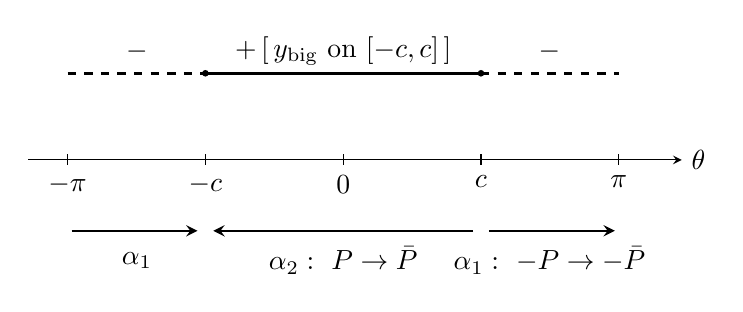
\begin{tikzpicture}[x=1cm,y=1cm,>=stealth]
  % theta axis
  \draw[->] (-4,0) -- (4.3,0) node[right] {$\theta$};
  \draw (3.5,0.07) -- (3.5,-0.07) node[below] {$\pi$};
  \draw (-3.5,0.07) -- (-3.5,-0.07) node[below] {$-\pi$};
  \draw (1.75,0.07) -- (1.75,-0.07) node[below] {$c$};
  \draw (-1.75,0.07) -- (-1.75,-0.07) node[below] {$-c$};
  \draw (0,0.07) -- (0,-0.07) node[below] {$0$};
  % big branch: Samart's signed open chain
  \draw[very thick] (-1.75,1.1) -- (1.75,1.1);
  \node at (0,1.38) {$+\,[\,y_{\mathrm{big}}\text{ on }[-c,c]\,]$};
  \draw[very thick,dashed] (-3.5,1.1) -- (-1.75,1.1);
  \draw[very thick,dashed] (1.75,1.1) -- (3.5,1.1);
  \node at (-2.62,1.38) {$-$};
  \node at (2.62,1.38) {$-$};
  \fill (1.75,1.1) circle (1.2pt);
  \fill (-1.75,1.1) circle (1.2pt);
  % small branch: compensating arcs beta_0 = alpha_1 + alpha_2
  \draw[thick,->] (1.65,-0.9) -- (-1.65,-0.9);
  \node at (0,-1.28) {$\alpha_2:\ P\to\bar P$};
  \draw[thick,->] (1.85,-0.9) -- (3.45,-0.9);
  \draw[thick,->] (-3.45,-0.9) -- (-1.85,-0.9);
  \node at (2.62,-1.28) {$\alpha_1:\ -P\to-\bar P$};
  \node at (-2.62,-1.28) {$\alpha_1$};
\end{tikzpicture}
\caption{The closed anti-invariant cycle $C'=\tilde\gamma+\beta_0$ on the
torus $|x|=1$ (schematic). Top: Samart's signed open chain $\tilde\gamma$ on
the big branch (weight $+$ on $[-c,c]$, weight $-$ on the outer arcs), with
branch jumps at the fold points $\theta=\pm c$. Bottom: the compensating
small-branch arcs $\beta_0=\alpha_1+\alpha_2$; their boundary is the negative
of $\partial\tilde\gamma$, so $C'$ is closed, and complex conjugation shows
$c(C')=-C'$.}
\label{fig:chain}
\end{figure}

\subsection{Homology class: \texorpdfstring{$C'=2\gamma^-$}{C'=2g-} (certified)}
\label{subsec:class}

In genus $1$ with $\Delta<0$, $H_1(E,\Z)^-=\Z\gamma^-$, the pairing with
$\omega$ is injective (period lattice isomorphism), and
$\period(\gamma^-)=\pm w_{\mathrm{anti}}$ with
$w_{\mathrm{anti}}=2i\,\Imz\,\omega_2$. Therefore
$\period(C')/w_{\mathrm{anti}}$ is \emph{a priori} a non-zero integer.

The computation (\texttt{code/n1\_certify.py}, mpmath at $60$ and $80$
digits, cross-checked against PARI \texttt{11.a3} \texttt{E.omega}) gives
\begin{equation}\label{eq:period}
  \period(C')=I_{\mathrm{signed}}+A_{s,\mathrm{outer}}-A_{s,\mathrm{inner}}
  =-5.8352664677539809\ldots\,i,
\end{equation}
\[
  \frac{\period(C')}{w_{\mathrm{anti}}}=1.9999999999999999\ldots,\qquad
  \big|\period(C')-2w_{\mathrm{anti}}\big|=2.5\times10^{-16},
\]
where $I_{\mathrm{signed}}=-2.917633233876990458\ldots i$ is the period of
the open signed chain and $A_{s,\mathrm{outer}},A_{s,\mathrm{inner}}$ are the
period integrals of the compensating arcs; the $60$- and $80$-digit runs
agree, the residual error coming from the $1/\sqrt\theta$ endpoint
singularity at $\theta=0$. A-priori integrality $+$ distance-to-nearest-integer
$2.5\times10^{-16}\ll 1$ imply the certified equality
\[
  \boxed{\class(C')=2\,\gamma^-}.
\]
(As a by-product one obtains the two independent period identities
$I_{\mathrm{signed}}=w_{\mathrm{anti}}$ and
$A_{s,\mathrm{inner}}-A_{s,\mathrm{outer}}=-w_{\mathrm{anti}}$.)

\begin{remark}
This corrects an earlier (``second wave'') claim that $\tilde\gamma$ itself is
a generator of $H_1(E,\Z)^-$ (winding number $n=1$): $\tilde\gamma$ is an
open chain; the correct closed cycle $C'$ has winding number $2$. For
contrast, the naive loop integral $I_{\mathrm{loop}}=-0.47447\ldots i$ is not
even the period of any integral cycle (ratio $0.16262\ldots$ to
$w_{\mathrm{anti}}$).
\end{remark}

\subsection{The regulator identity along the closed chain}

On $|x|=1$, $\eta(x,y)=\log|x|\,d\arg y-\log|y|\,d\arg x=-\log|y|\,d\theta$,
and since the product of the two roots is $x^3$ of modulus $1$,
$\log|y_{\mathrm{big}}|=-\log|y_{\mathrm{small}}|$ pointwise. Writing
$J_1=\int_0^c\log|y_s|\,d\theta$ and $J_2=\int_c^\pi\log|y_s|\,d\theta$,
direct computation gives
\[
  \int_{\tilde\gamma}\eta=2(J_1-J_2)
  =\underbrace{(2J_1)}_{\alpha_2}+\underbrace{(-2J_2)}_{\alpha_1}
  =\int_{\beta_0}\eta,
\]
hence the \emph{exact} identity
\begin{equation}\label{eq:double}
  \int_{C'}\eta=2\int_{\tilde\gamma}\eta.
\end{equation}

\subsection{Regulator constants: Bloch, Brunault, Bertin}

The divisor algebra (projective computation on the cubic model, Abel's
principal-divisor test passed) gives, with $A=(0,0)$ the $5$-torsion point
and $O=[0:1:0]$,
\[
  \divisor(x)=[A]+[2A]-[O]-[3A],\qquad
  \divisor(y)=3[A]-2[O]-[3A],
\]
hence the diamond product
\[
  (x)\diamond(y)=6(O)+5(A)-5(2A),\qquad
  D_E\big((x)\diamond(y)\big)=5D_E(P)-5D_E(2P).
\]
The elliptic dilogarithm values (mpmath, $60$ digits; lattice basis
$(w_1,w_1-w_2)$ so that $\tau=0.5+0.2299i$; $z(P)=0.6w_1$, $z(2P)=0.2w_1$
from PARI \texttt{ellpointtoz}):
\[
  D_E(P)=0.1911937370843316957549544343121738161012\ldots
\]
The two key identities (both verified to $40$ digits, and both theorems in
the literature) are
\begin{itemize}
  \item \textbf{Brunault's coefficient} \cite{Brunault}*{(3.151)}:
  $D_E(P)=\dfrac{2\pi}{5}b_{11}=\dfrac{11}{10\pi}L(E,2)$, i.e.\
  $L(E,2)=\frac{10\pi}{11}D_E(P)$;
  \item \textbf{Bertin's exotic relation} \cite{Bertin}:
  $D_E(2P)=\frac32D_E(P)$ (note $\tfrac32$, not the naive $2$).
\end{itemize}
Closing the loop:
\[
  5D_E(P)-5D_E(2P)=5\Bigl(1-\tfrac32\Bigr)D_E(P)=-\tfrac52D_E(P)=-\pi b_{11}.
\]
By Bloch's theorem \cite{Bloch} in its original normalisation
$r(\{f,g\})=\frac{1}{2\pi}\int_\gamma\eta(f,g)$ ($\gamma$ generating
$H_1(E,\Z)^-$) one has $\pi\,r(\{f,g\})=D_E((f)\diamond(g))$
\cite{Touafek}*{Thm.~1}, i.e.\
\[
  \int_{\gamma^-}\eta=\pm 2\,D_E\big((x)\diamond(y)\big)=\mp 2\pi b_{11},
\]
the sign depending on orientation (Brunault, Remarque~20: $D_E$ depends on
the orientation of $E(\R)$ and is defined only up to sign). In fact Brunault's
(3.210)--(3.211), quoting Bertin, already give
$|r_{\gamma^-}\{x,y\}|=\frac{5}{2\pi}D_E(P)=b_{11}$ directly: the regulator
side is a proved theorem; the gap closed here is the identification of Boyd's
split-integral chain with the closed cycle in $H_1(E,\Z)^-$.

\subsection{Synthesis}

\begin{theorem}[(C3)]\label{thm:C3}
$I_{\mathrm{split}}=b_{11}$.
\end{theorem}

\begin{proof}
By \eqref{eq:double} and $\class(C')=2\gamma^-$
(\S\ref{subsec:class}),
\[
  \int_{\tilde\gamma}\eta=\frac12\int_{C'}\eta
  =\frac12\cdot 2\cdot(\pm 2\pi b_{11})=\pm 2\pi b_{11}.
\]
The sign is pinned by a single numerical evaluation:
$\int_{\tilde\gamma}\eta=+0.9559686854\ldots=+2\pi b_{11}$ with $b_{11}>0$.
Finally, by the structural identity
$I_{\mathrm{split}}=\frac{1}{2\pi}\int_{\tilde\gamma}\eta$
(Section~\ref{sec:family}),
\[
  I_{\mathrm{split}}=b_{11}. \qedhere
\]
\end{proof}

%=====================================================================
\section{Numerical certification}
\label{sec:cert}

\subsection{Certified computations}

All floating-point computations are performed with mpmath at $60$--$300$
digits and cross-checked with PARI/GP 2.15.5:

\begin{itemize}
  \item \textbf{The constant $b_{11}$} (\texttt{code/b11.py}): from the exact
  integer coefficients of $f_{11}=\eta(\tau)^2\eta(11\tau)^2$ (truncated
  convolution of the squared Euler function) via the approximate functional
  equation for weight $2$, root number $+1$:
  \[
    b_{11}=\Lambda(f,2)=\sum_{n\ge1}a_n\Big[e^{-t_n}\Big(\frac1{t_n}
    +\frac1{t_n^2}\Big)+E_1(t_n)\Big],\qquad t_n=\frac{2\pi n}{\sqrt{11}},
  \]
  with terms decaying like $e^{-1.894n}$; $200$ terms suffice for $300$
  digits.
  \item \textbf{(C3) to $149$ digits} (\texttt{code/attack3.py}):
  \[
    I_{\mathrm{split}}
    =0.152147141725918049486227297478634495628143589164226122809889823882023289695302776676\ldots,
  \]
  \[
    |I_{\mathrm{split}}-b_{11}|=4.85\times10^{-149}.
  \]
  \item \textbf{(C1)/(C2) reproduced} to $52$ digits
  (\texttt{code/attack1.py}): $\|m-7b_{11}\|\approx5.0\times10^{-53}$,
  $\|m-5b_{11}\|\approx3.6\times10^{-53}$.
  \item \textbf{Period certification} (\texttt{code/n1\_certify.py},
  \texttt{code/n1\_certify.gp}): \eqref{eq:period} computed independently at
  $60$ and $80$ digits with identical results; each arc integral $A_s$ is
  stable to $24$ digits across $40/60/80$-digit runs; $w_{\mathrm{anti}}$
  taken from PARI \texttt{E.omega} for \texttt{11.a3}. The integrality
  argument has an a-priori gap of $1$ against a residual of
  $2.5\times10^{-16}$.
  \item \textbf{Exact algebraic checks}: group law and torsion
  (\texttt{code/torsion.py}, \texttt{code/endpoint\_torsion2.py}) use exact
  rational arithmetic over $\Q$, $\Q(\sqrt2)$, $\Q(\zeta_8)$---no numerical
  approximation; the model constant $\kappa=1$ is fixed by the discrete
  candidates $\kappa^{12}=\Delta_{\mathrm{quartic}}/\Delta_{\min}=2^a11^b$
  plus $50$-digit agreement.
  \item \textbf{PARI/GP cross-checks}: \texttt{verify\_family.gp},
  \texttt{verify\_ratios.gp} (family conductors, $j$-invariants, $b$-values
  vs.\ \texttt{lfun} to $50+$ digits), \texttt{winding.gp},
  \texttt{dilog.gp}, \texttt{k53.gp}, \texttt{k53b.gp},
  \texttt{kfamily\_torsion.gp}.
\end{itemize}

\subsection{Level of rigour: interval certification}
\label{subsec:rigour}

The integer identification in \S\ref{subsec:class} has been made fully
interval-rigorous (\texttt{code/n1\_interval.py}, python-flint/Arb ball
arithmetic \cite{Arb}, $300$-bit working precision; output
\texttt{notes/attack10-interval.txt}).  All three arc integrals were
recomputed with Arb's certified adaptive Gauss--Legendre integration:
\begin{itemize}
  \item the endpoint singularity $u\sim\sqrt{\theta}$ at $\theta=0$ is removed
  by the substitution $\theta=\pm t^{2}$; the substituted integrand is
  analytic on the disc $|t|\le\rho=0.6$ (the nonzero zeros of $D(t^{2})$
  satisfy $|\theta_{j}|\ge1.2188$, certified by Newton--Rouch\'e isolation of
  the roots of $z^{4}-4z^{3}+2z^{2}+1$), and the tip $[0,\delta]$, $\delta=\rho/5$,
  is summed by the Cauchy estimate $\int_{0}^{\delta}f=a_{0}\delta+R$,
  $|R|\le H\delta^{3}/3$, where $H$ is derived from
  $M=\max_{|t|=\rho}|f|=1.3075\ldots$, itself certified by covering the
  circle with $4096$ balls (per-tip radius $2.18\times10^{-3}$);
  \item $D(\theta)$ crosses the negative real axis once on $(c,\pi)$ and once
  on $(-\pi,-c)$, where the principal square root is not analytic: the arcs
  are subdivided adaptively, on each piece either $\sqrt{D}$ or $i\sqrt{-D}$
  is certified analytic by ball evaluation, and the overall sign is
  propagated across the nodes by a certified matching test;
  \item $w_{\mathrm{anti}}$ is certified independently of PARI: the roots of
  $4x^{3}-4x^{2}+1$ are isolated by Newton iteration plus a Rouch\'e
  certificate, and Carlson's $R_{F}$ gives
  $w_{\mathrm{real}}=6.34604652139776710844397\ldots$ ($\pm2.3\times10^{-45}$)
  and $w_{\mathrm{anti}}=2.91763323387699045866178\ldots i$
  ($\pm6.8\times10^{-47}$), agreeing with PARI to $45$ digits.
\end{itemize}
The resulting ratio ball is
$[-2.00\pm3.13\times10^{-3}]+[\pm2.99\times10^{-3}]\,i$: it contains $-2$ and
$|\mathrm{ratio}+2|\le4.33\times10^{-3}<1/2$.  The a-priori integrality of
\S\ref{subsec:class} therefore upgrades to the exact equality
$\mathrm{period}(C')=-2\,w_{\mathrm{anti}}$ (the sign is an orientation
convention, $|\class(C')|=2\gamma^{-}$), and Theorem~\ref{thm:C3} holds
without any certification-level caveat.

%=====================================================================
\section{Conjectures}
\label{sec:conjectures}

The family identities established numerically here are stated as conjectures
pending analytic proof:

\begin{conjecture}\label{conj:family}
For $S_k=y^2+(x^2+kx+1)y+x^3$ with $|k|\ge 2$, there is a small rational
number $r_k$ such that
\[
  m(S_k)=r_k\,|L'(E_k,0)|.
\]
Confirmed numerically: $r_2=2$, $r_3=1$ (60 digits), and
$r_{-4}=\tfrac72$ (conductor $37$), $r_{-5}=\tfrac14$ (conductor $359$),
$r_{-6}=\tfrac18$ (conductor $997$) (25 digits each).
\end{conjecture}

The last three deserve emphasis as \emph{predicted then confirmed}: the
structural theorem (Theorem~\ref{thm:family}) predicted, from the
torus-intersection trichotomy, that $k=-4,-5,-6$ must satisfy Boyd-type
identities with specific small rationals, and the subsequent computation hit
the predicted values. Note that $S_{-4}$ and $S_2$ share conductor $37$,
yielding Rodr\'iguez Villegas--type rational relations \cite{RV,LalinRam}
between two different polynomial models of the same curve.

\begin{conjecture}[Samart's conductor-$17$ analogue, independently confirmed]
For $k=1$ (conductor $17$), $\tilde n(1)=b_{17}$, i.e.\ the signed
split-integral of $S_1$ equals $|L'(E_{17},0)|$ (60 digits).
\end{conjecture}

\begin{remark}
By Theorem~\ref{thm:k53}, no such conjecture can be formulated for $k=-1$
(conductor $53$): the anti-invariant cycle on the torus does not exist and
$x,y$ are not modular units.
\end{remark}

%=====================================================================
\appendix
\section{Reproduction code}
\label{app:code}

All scripts live in \texttt{code/}; raw outputs in
\texttt{notes/attack*-results.txt}. Dependencies: Python 3.12 with mpmath and
sympy; PARI/GP 2.15.5; python-flint 0.9.0 (Arb) for the interval certification.

\begin{center}
\begin{tabular}{@{}ll@{}}
\toprule
File & Purpose\\
\midrule
\texttt{b11.py} & $b_{11}=L'(E_{11},0)$ to 300 digits via approximate functional equation\\
\texttt{attack1.py} & reproduce (C1), (C2) to 52 digits\\
\texttt{attack2.py} & $m(S_0)$, PSLQ negative results\\
\texttt{attack3.py} & (C3) to 149 digits\\
\texttt{torsion.py} & exact group law: $5A=O$, modular units\\
\texttt{endpoint\_torsion2.py} & exact check: endpoint $P$ non-torsion\\
\texttt{boundary\_torsion.py} & boundary-divisor torsion analysis\\
\texttt{closedness\_check.py} & $\tilde n=-I_{\mathrm{split}}$, regulator $=2\pi I_{\mathrm{split}}$\\
\texttt{ntilde\_family.py} & $\tilde n(k)$ family table, 50--80 digits\\
\texttt{b\_family.py} & $b_N$ for the family via point counting\\
\texttt{winding.py} / \texttt{winding.gp} & period pairings, winding-number heuristics\\
\texttt{dilog.py} / \texttt{dilog.gp} & elliptic dilogarithm $D_E(P)$, Brunault/Bertin constants\\
\texttt{k53\_attack.py} & conductor-$53$ obstruction analysis\\
\texttt{k53.gp} / \texttt{k53b.gp} & PARI checks for \texttt{53.a1}\\
\texttt{kneg\_m.py} & $m(S_k)$ for $k=-4,-5,-6$ (predicted identities)\\
\texttt{n1\_certify.py} / \texttt{n1\_certify.gp} & certification of $\class(C')=2\gamma^-$\\
\texttt{n1\_interval.py} & Arb ball-arithmetic ironclad proof of the period ratio\\
\texttt{verify\_family.gp} & PARI cross-check of family conductors and $j$-invariants\\
\texttt{verify\_ratios.gp} & PARI \texttt{lfun} cross-check of ratios\\
\texttt{kfamily\_torsion.gp} & torsion subgroups and $\operatorname{ord}(0,0)$ for the family\\
\bottomrule
\end{tabular}
\end{center}

Reproduction:
\begin{verbatim}
cd code && python b11.py && python attack1.py && python attack2.py \
  && python attack3.py && python torsion.py && python endpoint_torsion2.py \
  && python boundary_torsion.py && python closedness_check.py \
  && python ntilde_family.py && python b_family.py && python winding.py \
  && python dilog.py && python k53_attack.py && python kneg_m.py \
  && python n1_certify.py
.venv/Scripts/python n1_interval.py    # Arb interval certification (needs python-flint)
gp -q verify_family.gp && gp -q verify_ratios.gp
gp -q winding.gp && gp -q dilog.gp
gp -q k53.gp && gp -q k53b.gp && gp -q kfamily_torsion.gp
\end{verbatim}

%=====================================================================
\begin{thebibliography}{99}

\bibitem{Bertin}
M.-J. Bertin,
\emph{Mesure de Mahler et r\'egulateur elliptique: preuve de deux relations
``exotiques''},
in: Number theory, CRM Proc. Lecture Notes \textbf{36}, Amer. Math. Soc.,
Providence, RI, 2004, pp.~1--12.

\bibitem{BertinLalin}
M.-J. Bertin and M. Lal\'in,
\emph{Mahler measure of multivariable polynomials},
in: Women in Numbers 2: Research Directions in Number Theory,
Contemp. Math. \textbf{606}, Amer. Math. Soc., Providence, RI, 2013,
pp.~125--147.

\bibitem{Bloch}
S.~J. Bloch,
\emph{Higher regulators, algebraic $K$-theory, and zeta functions of
elliptic curves},
CRM Monograph Series \textbf{11}, Amer. Math. Soc., Providence, RI, 2000.

\bibitem{Boyd98}
D.~W. Boyd,
\emph{Mahler's measure and special values of $L$-functions},
Experiment. Math. \textbf{7} (1998), no.~1, 37--82.

\bibitem{Brunault}
F.~Brunault,
\emph{\'Etude de la valeur en $s=2$ de la fonction $L$ d'une courbe
elliptique},
th\`ese, Universit\'e Paris 7 -- Denis Diderot, 2005.

\bibitem{BrunaultBSMF}
F.~Brunault,
\emph{Valeur en $2$ de fonctions $L$ de formes modulaires de poids $2$:
th\'eor\`eme de Beilinson explicite},
Bull. Soc. Math. France \textbf{135} (2007), no.~2, 215--246.

\bibitem{Deninger}
C.~Deninger,
\emph{Deligne periods of mixed motives, $K$-theory and the entropy of
certain $\Z^n$-actions},
J. Amer. Math. Soc. \textbf{10} (1997), no.~2, 259--281.

\bibitem{Arb}
F.~Johansson,
\emph{Arb: efficient arbitrary-precision midpoint-radius interval
arithmetic},
IEEE Trans. Comput. \textbf{66} (2017), no.~8, 1281--1292.

\bibitem{mpmath}
F.~Johansson et al.,
\emph{mpmath: a Python library for arbitrary-precision floating-point
arithmetic}, \url{http://mpmath.org/}.

\bibitem{LalinRam}
M.~Lal\'in and F.~Ramamonjisoa,
\emph{The Mahler measure of a Weierstrass form},
Int. J. Number Theory \textbf{13} (2017), no.~8, 2195--2214.

\bibitem{LSZ}
M.~Lal\'in, D.~Samart and W.~Zudilin,
\emph{Further explorations of Boyd's conjectures and a conductor $21$
elliptic curve},
J. Lond. Math. Soc. (2) \textbf{93} (2016), no.~2, 341--360.

\bibitem{LMFDB}
The LMFDB Collaboration,
\emph{The $L$-functions and Modular Forms Database},
\url{https://www.lmfdb.org}, 2026.

\bibitem{PARI}
The PARI~Group,
\emph{PARI/GP version \texttt{2.15.5}},
Univ. Bordeaux, 2024, \url{http://pari.math.u-bordeaux.fr/}.

\bibitem{RV}
F.~Rodr\'iguez Villegas,
\emph{Modular Mahler measures. I},
in: Topics in number theory (University Park, PA, 1997),
Math. Appl. \textbf{467}, Kluwer Acad. Publ., Dordrecht, 1999, pp.~17--48.

\bibitem{RZ15}
M.~Rogers and W.~Zudilin,
\emph{From $L$-series of elliptic curves to Mahler measures},
Compos. Math. \textbf{148} (2012), no.~2, 385--414.

\bibitem{Samart2023}
D.~Samart,
\emph{Mahler measure of a non-reciprocal family of elliptic curves},
Q. J. Math. \textbf{74} (2023), no.~4, 1187--1208.

\bibitem{Smyth}
C.~J. Smyth,
\emph{On measures of polynomials in several variables},
Bull. Austral. Math. Soc. \textbf{23} (1981), no.~1, 49--63.

\bibitem{Touafek}
N.~Touafek,
\emph{From the elliptic regulator to exotic relations},
An. \c Stiin\c t. Univ. ``Ovidius'' Constan\c ta Ser. Mat. \textbf{16}
(2008), no.~2, 117--126.

\bibitem{Zudilin}
W.~Zudilin,
\emph{Regulator of modular units and Mahler measures},
Math. Proc. Cambridge Philos. Soc. \textbf{156} (2014), no.~2, 313--326.

\end{thebibliography}

\end{document}
